\documentclass[14pt]{extbook}
\usepackage{multicol, enumerate, enumitem, hyperref, color, soul, setspace, parskip, fancyhdr} %General Packages
\usepackage{amssymb, amsthm, amsmath, bbm, latexsym, units, mathtools} %Math Packages
\everymath{\displaystyle} %All math in Display Style
% Packages with additional options
\usepackage[headsep=0.5cm,headheight=12pt, left=1 in,right= 1 in,top= 1 in,bottom= 1 in]{geometry}
\usepackage[usenames,dvipsnames]{xcolor}
\usepackage{dashrule}  % Package to use the command below to create lines between items
\newcommand{\litem}[1]{\item#1\hspace*{-1cm}\rule{\textwidth}{0.4pt}}
\pagestyle{fancy}
\lhead{Progress Quiz 4}
\chead{}
\rhead{Version C}
\lfoot{6286-1986}
\cfoot{}
\rfoot{Fall 2020}
\begin{document}

\begin{enumerate}
\litem{
Solve the radical equation below. Then, choose the interval(s) that the solution(s) belongs to.\[ \sqrt{25 x^2 - 64} - \sqrt{0 x} = 0 \]\begin{enumerate}[label=\Alph*.]
\item \( x \in [-5.6,-0.6] \)
\item \( \text{All solutions lead to invalid or complex values in the equation.} \)
\item \( x_1 \in [-0.4, 4.6] \text{ and } x_2 \in [-0.4,4.6] \)
\item \( x \in [-0.4,4.6] \)
\item \( x_1 \in [-5.6, -0.6] \text{ and } x_2 \in [-0.4,4.6] \)

\end{enumerate} }
\litem{
Choose the equation of the function graphed below.
\begin{center}
    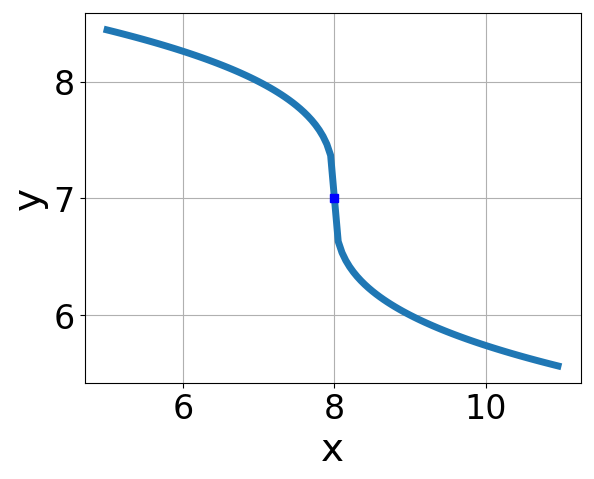
\includegraphics[width=0.5\textwidth]{../Figures/radicalGraphToEquationC.png}
\end{center}
\begin{enumerate}[label=\Alph*.]
\item \( f(x) = - \sqrt[3]{x + 10} + 5 \)
\item \( f(x) = - \sqrt[3]{x - 10} + 5 \)
\item \( f(x) = \sqrt[3]{x + 10} + 5 \)
\item \( f(x) = \sqrt[3]{x - 10} + 5 \)
\item \( \text{None of the above} \)

\end{enumerate} }
\litem{
Solve the radical equation below. Then, choose the interval(s) that the solution(s) belongs to.\[ \sqrt{-25 x^2 + 24} - \sqrt{25 x} = 0 \]\begin{enumerate}[label=\Alph*.]
\item \( x \in [0.6,3.6] \)
\item \( \text{All solutions lead to invalid or complex values in the equation.} \)
\item \( x_1 \in [0.6, 3.6] \text{ and } x_2 \in [1.46,3] \)
\item \( x \in [-2.6,0.4] \)
\item \( x_1 \in [-2.6, 0.4] \text{ and } x_2 \in [0.52,0.88] \)

\end{enumerate} }
\litem{
Solve the radical equation below. Then, choose the interval(s) that the solution(s) belongs to.\[ \sqrt{-6 x - 2} - \sqrt{4 x + 2} = 0 \]\begin{enumerate}[label=\Alph*.]
\item \( x_1 \in [-0.73, -0.41] \text{ and } x_2 \in [-4.33,0.67] \)
\item \( \text{All solutions lead to invalid or complex values in the equation.} \)
\item \( x_1 \in [-0.42, -0.16] \text{ and } x_2 \in [-4.33,0.67] \)
\item \( x \in [-0.13,0.13] \)
\item \( x \in [-0.42,-0.16] \)

\end{enumerate} }
\litem{
What is the domain of the function below?\[ f(x) = \sqrt[3]{-3 x + 4} \]\begin{enumerate}[label=\Alph*.]
\item \( \text{The domain is } [a, \infty), \text{   where } a \in [0.78, 1.72] \)
\item \( (-\infty, \infty) \)
\item \( \text{The domain is } (-\infty, a], \text{   where } a \in [0.4, 1.3] \)
\item \( \text{The domain is } (-\infty, a], \text{   where } a \in [0.9, 2.9] \)
\item \( \text{The domain is } [a, \infty), \text{   where } a \in [0.33, 0.94] \)

\end{enumerate} }
\litem{
What is the domain of the function below?\[ f(x) = \sqrt[8]{7 x + 3} \]\begin{enumerate}[label=\Alph*.]
\item \( (-\infty, \infty) \)
\item \( (-\infty, a], \text{where } a \in [-4.33, -1.33] \)
\item \( (-\infty, a], \text{where } a \in [-1.43, 6.57] \)
\item \( [a, \infty), \text{where } a \in [-2.34, -0.43] \)
\item \( [a, \infty), \text{ where } a \in [-0.58, 0.81] \)

\end{enumerate} }
\litem{
Choose the graph of the equation below.\[ f(x) = - \sqrt[3]{x - 14} - 7 \]\begin{enumerate}[label=\Alph*.]
\begin{multicols}{2}\item 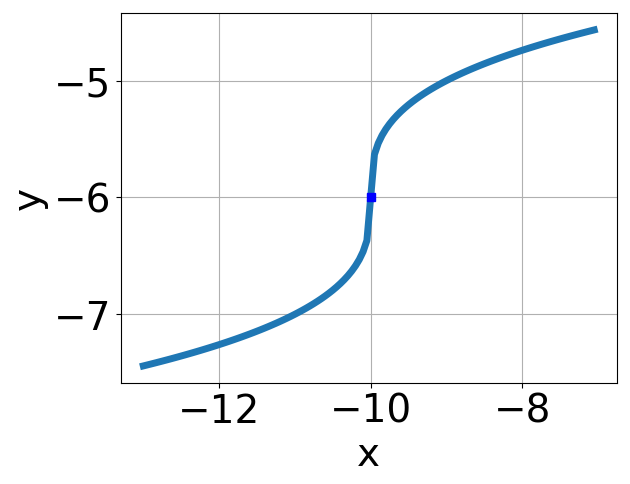
\includegraphics[width = 0.3\textwidth]{../Figures/radicalEquationToGraphAC.png}\item 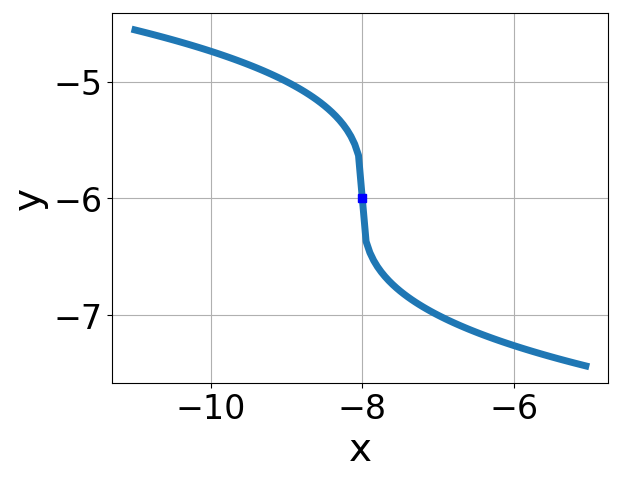
\includegraphics[width = 0.3\textwidth]{../Figures/radicalEquationToGraphBC.png}\item 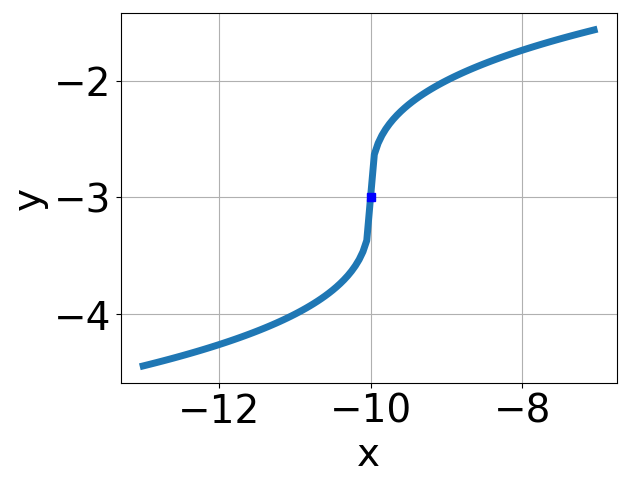
\includegraphics[width = 0.3\textwidth]{../Figures/radicalEquationToGraphCC.png}\item 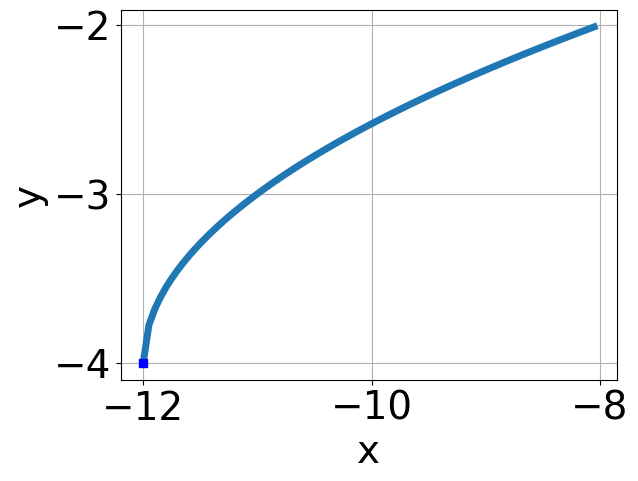
\includegraphics[width = 0.3\textwidth]{../Figures/radicalEquationToGraphDC.png}\end{multicols}\item None of the above.
\end{enumerate} }
\litem{
Solve the radical equation below. Then, choose the interval(s) that the solution(s) belongs to.\[ \sqrt{-2 x + 3} - \sqrt{-3 x - 3} = 0 \]\begin{enumerate}[label=\Alph*.]
\item \( x_1 \in [-3.6, -0.3] \text{ and } x_2 \in [-2.5,2.5] \)
\item \( \text{All solutions lead to invalid or complex values in the equation.} \)
\item \( x_1 \in [-6.7, -5.9] \text{ and } x_2 \in [-2.5,2.5] \)
\item \( x \in [-0.1,1.5] \)
\item \( x \in [-6.7,-5.9] \)

\end{enumerate} }
\litem{
Choose the graph of the equation below.\[ f(x) = - \sqrt{x - 8} + 4 \]\begin{enumerate}[label=\Alph*.]
\begin{multicols}{2}\item 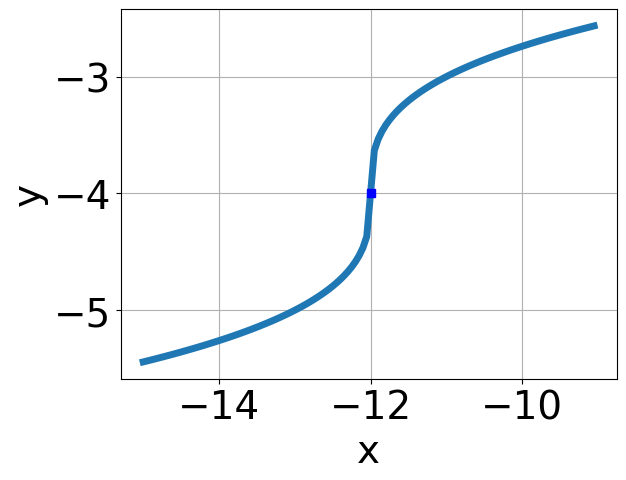
\includegraphics[width = 0.3\textwidth]{../Figures/radicalEquationToGraphCopyAC.png}\item 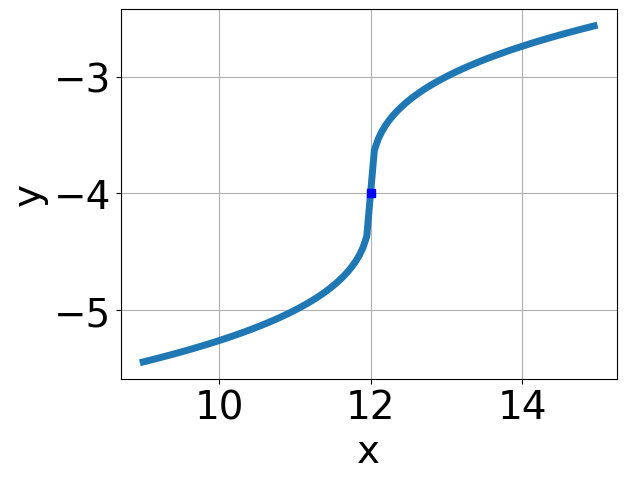
\includegraphics[width = 0.3\textwidth]{../Figures/radicalEquationToGraphCopyBC.png}\item 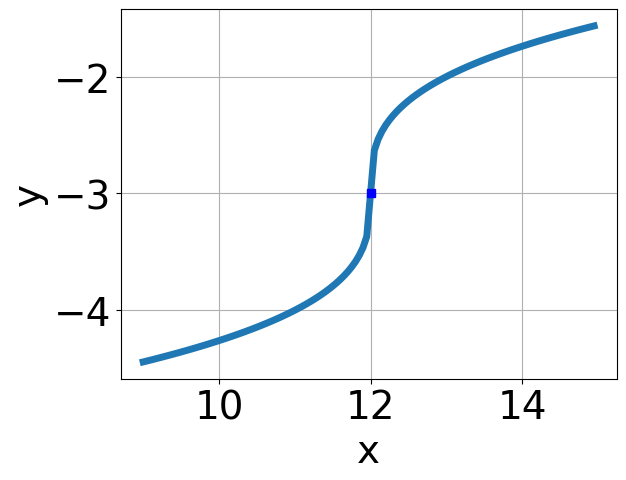
\includegraphics[width = 0.3\textwidth]{../Figures/radicalEquationToGraphCopyCC.png}\item 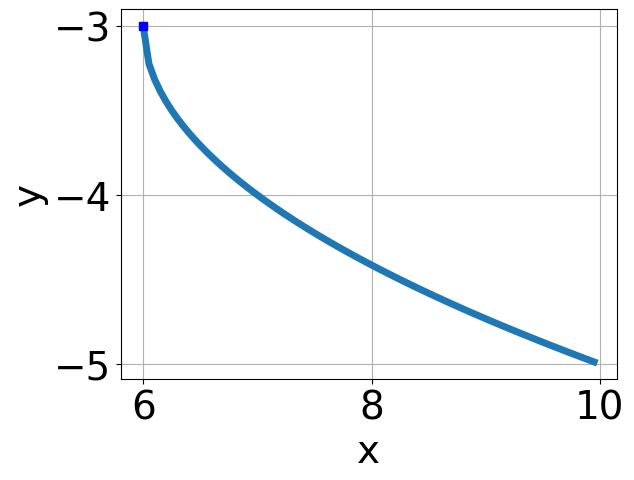
\includegraphics[width = 0.3\textwidth]{../Figures/radicalEquationToGraphCopyDC.png}\end{multicols}\item None of the above.
\end{enumerate} }
\litem{
Choose the equation of the function graphed below.
\begin{center}
    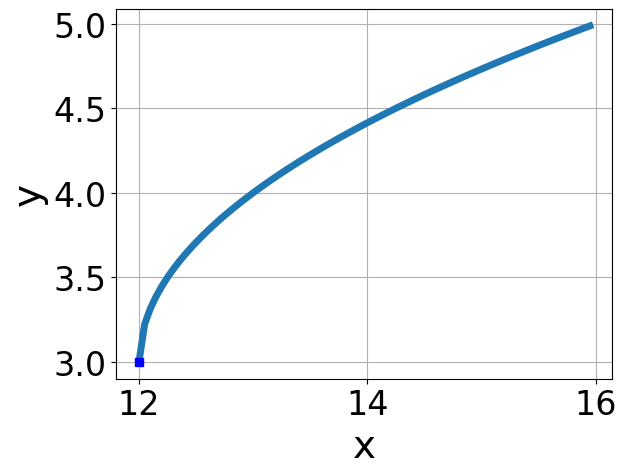
\includegraphics[width=0.5\textwidth]{../Figures/radicalGraphToEquationCopyC.png}
\end{center}
\begin{enumerate}[label=\Alph*.]
\item \( f(x) = \sqrt[3]{x + 12} + 3 \)
\item \( f(x) = \sqrt[3]{x - 12} + 3 \)
\item \( f(x) = - \sqrt[3]{x + 12} + 3 \)
\item \( f(x) = - \sqrt[3]{x - 12} + 3 \)
\item \( \text{None of the above} \)

\end{enumerate} }
\end{enumerate}

\end{document}